% Copyright (c) 2026 Islam Ibrahim. All rights reserved.

\documentclass[tikz,border=10pt]{standalone}
\usepackage[T1]{fontenc}
\usepackage{lmodern}
\usepackage{amsmath}
\usepackage{tikz}
\usetikzlibrary{arrows.meta}

\begin{document}
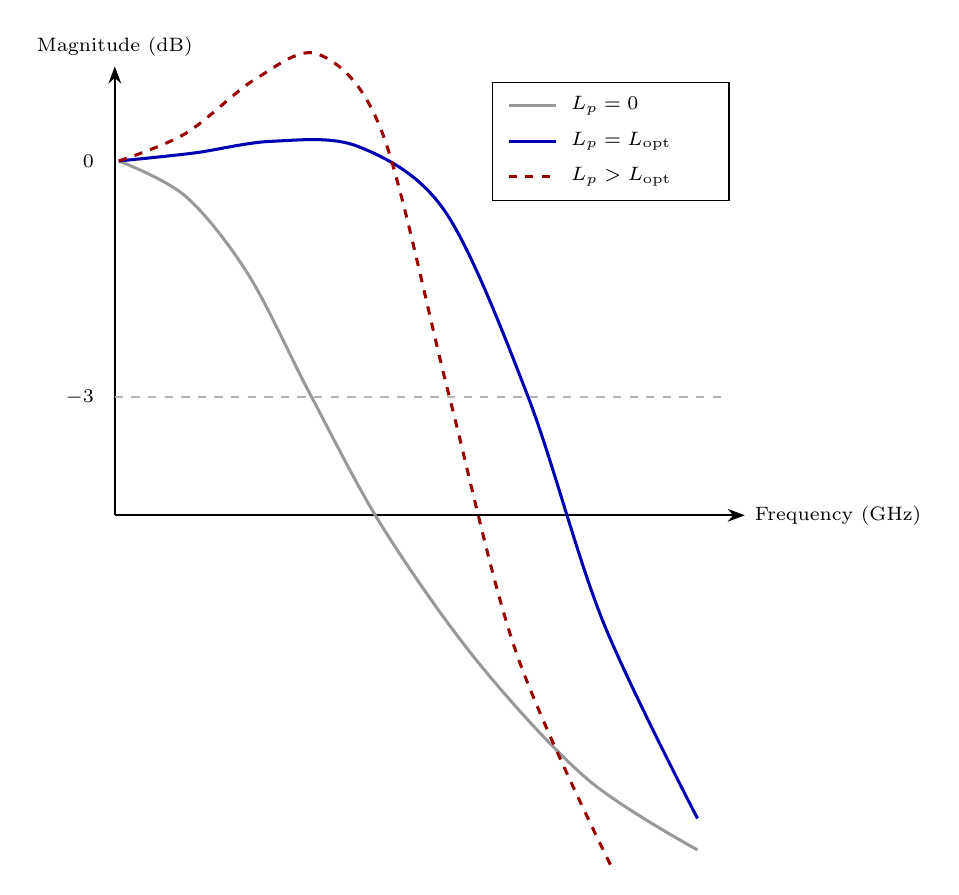
\begin{tikzpicture}[font=\small\rmfamily, >=Stealth,
  lbl/.style={font=\scriptsize\rmfamily},
  ax/.style={line width=0.7pt,->},
  seg/.style={line width=1.1pt},
]

% Axes
\draw[ax] (0,0.5) -- (0,6.2)
  node[above,lbl]{Magnitude (dB)};
\draw[ax] (0,0.5) -- (8.0,0.5)
  node[right,lbl]{Frequency (GHz)};
\node[lbl,left=4pt] at (0,5.0) {$0$};

% No peaking — first-order roll-off: -10*log10(1+(f/fc)^2)
\draw[seg,black!40] plot[smooth,tension=0.55] coordinates {
  (0.05,5.00) (0.9,4.55) (1.7,3.55) (2.5,2.00)
  (3.4,0.35) (4.6,-1.35) (6.0,-2.85) (7.4,-3.75)
};

% Optimal shunt peaking — second-order with slight peaking
\draw[seg,blue!70!black] plot[smooth,tension=0.55] coordinates {
  (0.05,5.00) (1.0,5.10) (2.0,5.25) (3.1,5.18)
  (4.2,4.35) (5.25,2.00) (6.2,-0.85) (7.4,-3.35)
};

% Over-peaking — second-order with excessive peaking
\draw[seg,red!60!black,dashed] plot[smooth,tension=0.55] coordinates {
  (0.05,5.00) (0.9,5.35) (1.8,6.05) (2.6,6.35)
  (3.4,5.35) (4.25,2.00) (5.1,-1.25) (6.3,-3.95)
};

% -3 dB reference line
\draw[line width=0.5pt,dashed,gray!60]
  (0,2.0) -- (7.8,2.0);
\node[lbl,left=4pt] at (0,2.0) {$-3$};

% Legend box — moved to top-right corner, clear of all curves
\draw[line width=0.4pt,fill=white,fill opacity=0.92] (4.8,6.0) rectangle (7.8,4.5);
\draw[seg,black!40]      (5.0,5.7) -- (5.6,5.7);
\node[lbl,right=2pt] at (5.6,5.7) {$L_p = 0$};
\draw[seg,blue!70!black] (5.0,5.25) -- (5.6,5.25);
\node[lbl,right=2pt] at (5.6,5.25) {$L_p = L_{\mathrm{opt}}$};
\draw[seg,red!60!black,dashed] (5.0,4.8) -- (5.6,4.8);
\node[lbl,right=2pt] at (5.6,4.8) {$L_p > L_{\mathrm{opt}}$};

\end{tikzpicture}
\end{document}
